\chapter{应用结果展示}  
\label{chp:display}

\begin{figure}
	\centering
	\begin{lstlisting}[language=Java]
package cn.mijack.rundroidtest;

public class MainActivity extends Activity implements View.OnClickListener {
	Button button1,button2,button3;
	Handler handler = new Handler() {
		public void handleMessage(Message msg) {
			if (msg.what == 1) {
				Toast.makeText(MainActivity.this, "handle", Toast.LENGTH_SHORT).show();
			}
		}
	};
	protected void onCreate(Bundle savedInstanceState) {
		super.onCreate(savedInstanceState);
		setContentView(R.layout.activity_main);
		button1 = findViewById(R.id.button1);
		button1.setOnClickListener(this);
		// button2、button3进行相同的操作
	}
	public void onClick(View view) {
		switch (view.getId()) {
			case R.id.button1:
				doHandleButton1();
				return;
				// button2、button3进行相同的操作
		}
	}
	public void doHandleButton1() {
		int fibonacci = doFibonacci(4);
		Toast.makeText(this, "fibonacci: " + fibonacci, Toast.LENGTH_SHORT).show();
	}
	private int doFibonacci(int i) {
		if (i < 0)    return -1;   
		if (i == 1 || i == 0)   return 1; 
		return doFibonacci(i - 1) + doFibonacci(i - 2);
	}
	public void doHandleButton2() {
		Message message = Message.obtain();
		message.what = 1;
		handler.sendMessage(message);
	}
	public void doHandleButton3() {
		Intent intent = new Intent(this, NewActivity.class);
		startActivity(intent);
	}
}\end{lstlisting}
%	\vspace{-9px}
	\caption{Example code for the Android execution model}
	\label{fig:code_demo}
\end{figure}

\section{函数调用图的构建结果展示}

斐波拉契数列


\eat{
	
	\begin{figure*}[ht]
		\centering
		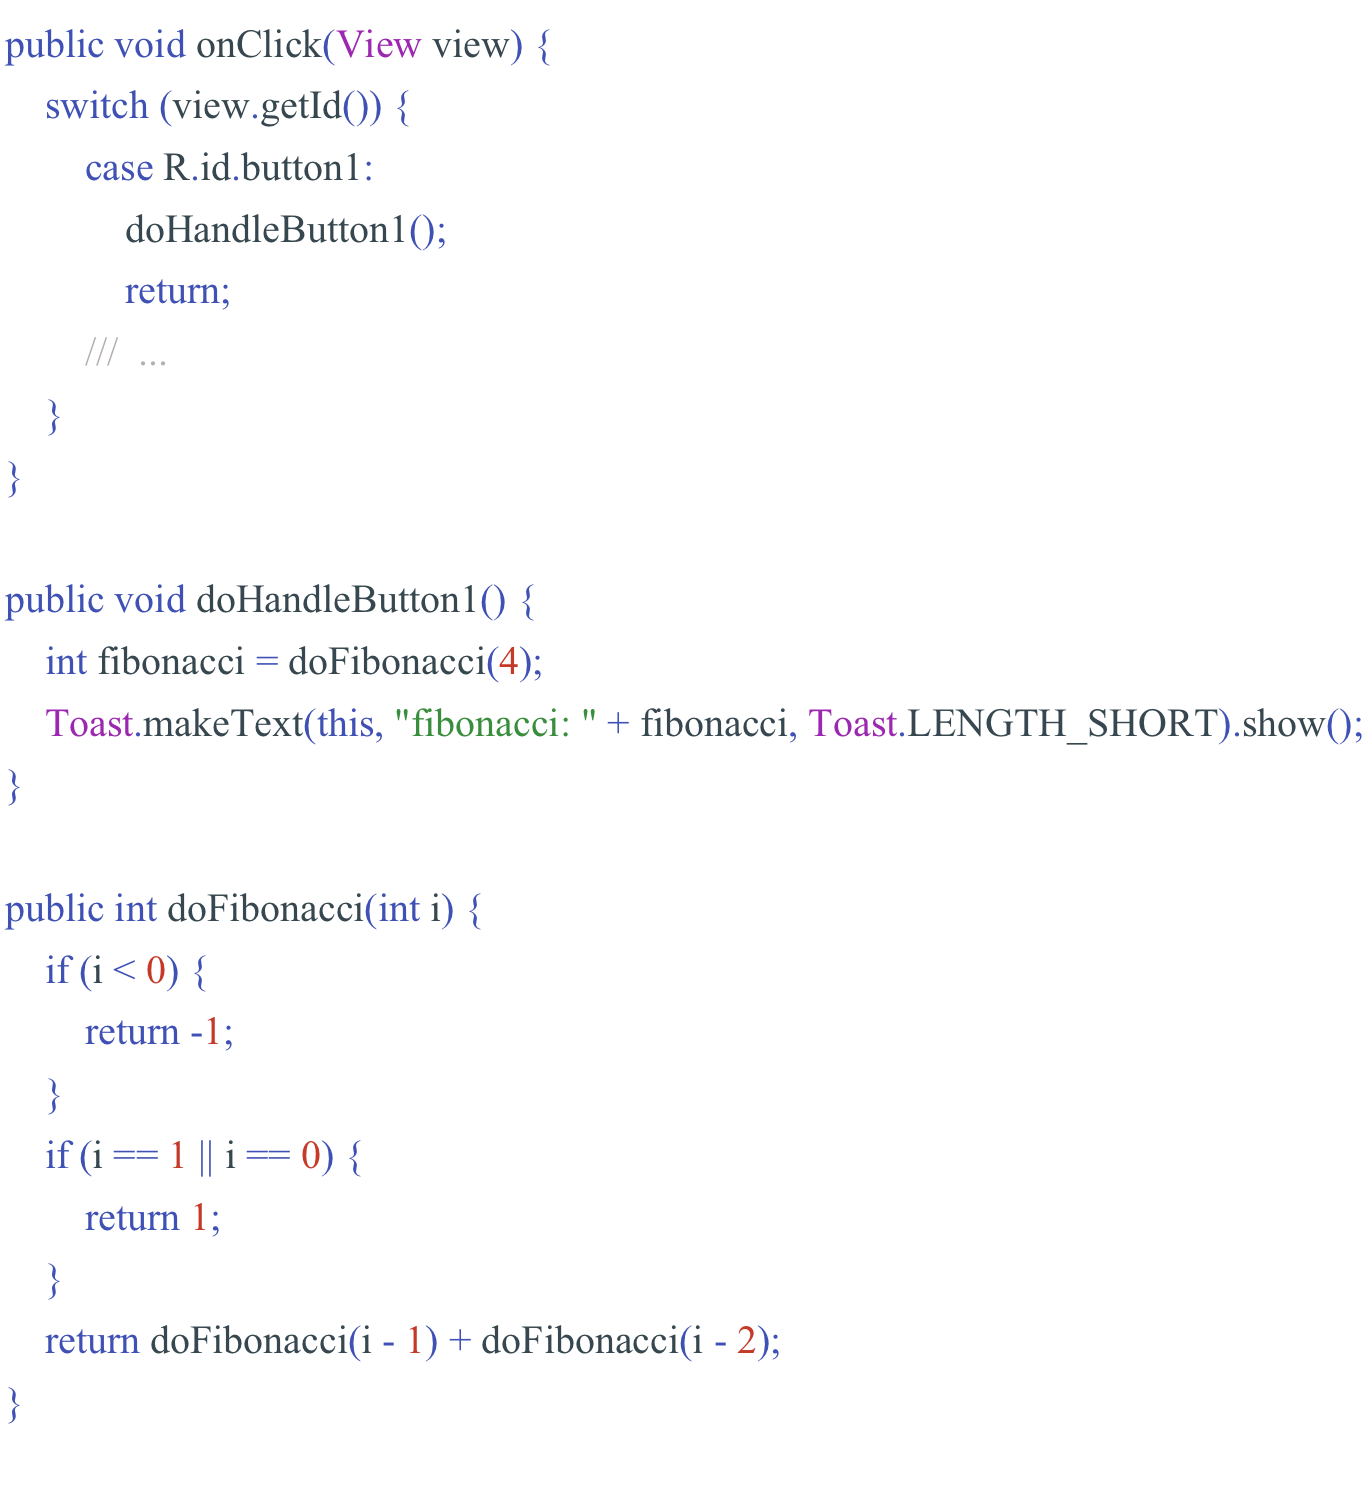
\includegraphics[width=0.65\textwidth]{./Figures/code-Fibonacci.png}
		\caption{斐波拉契数列相关的代码实现}
		\label{fig:code-Fibonacci}
\end{figure*}
}
\begin{figure*}[ht]
\centering
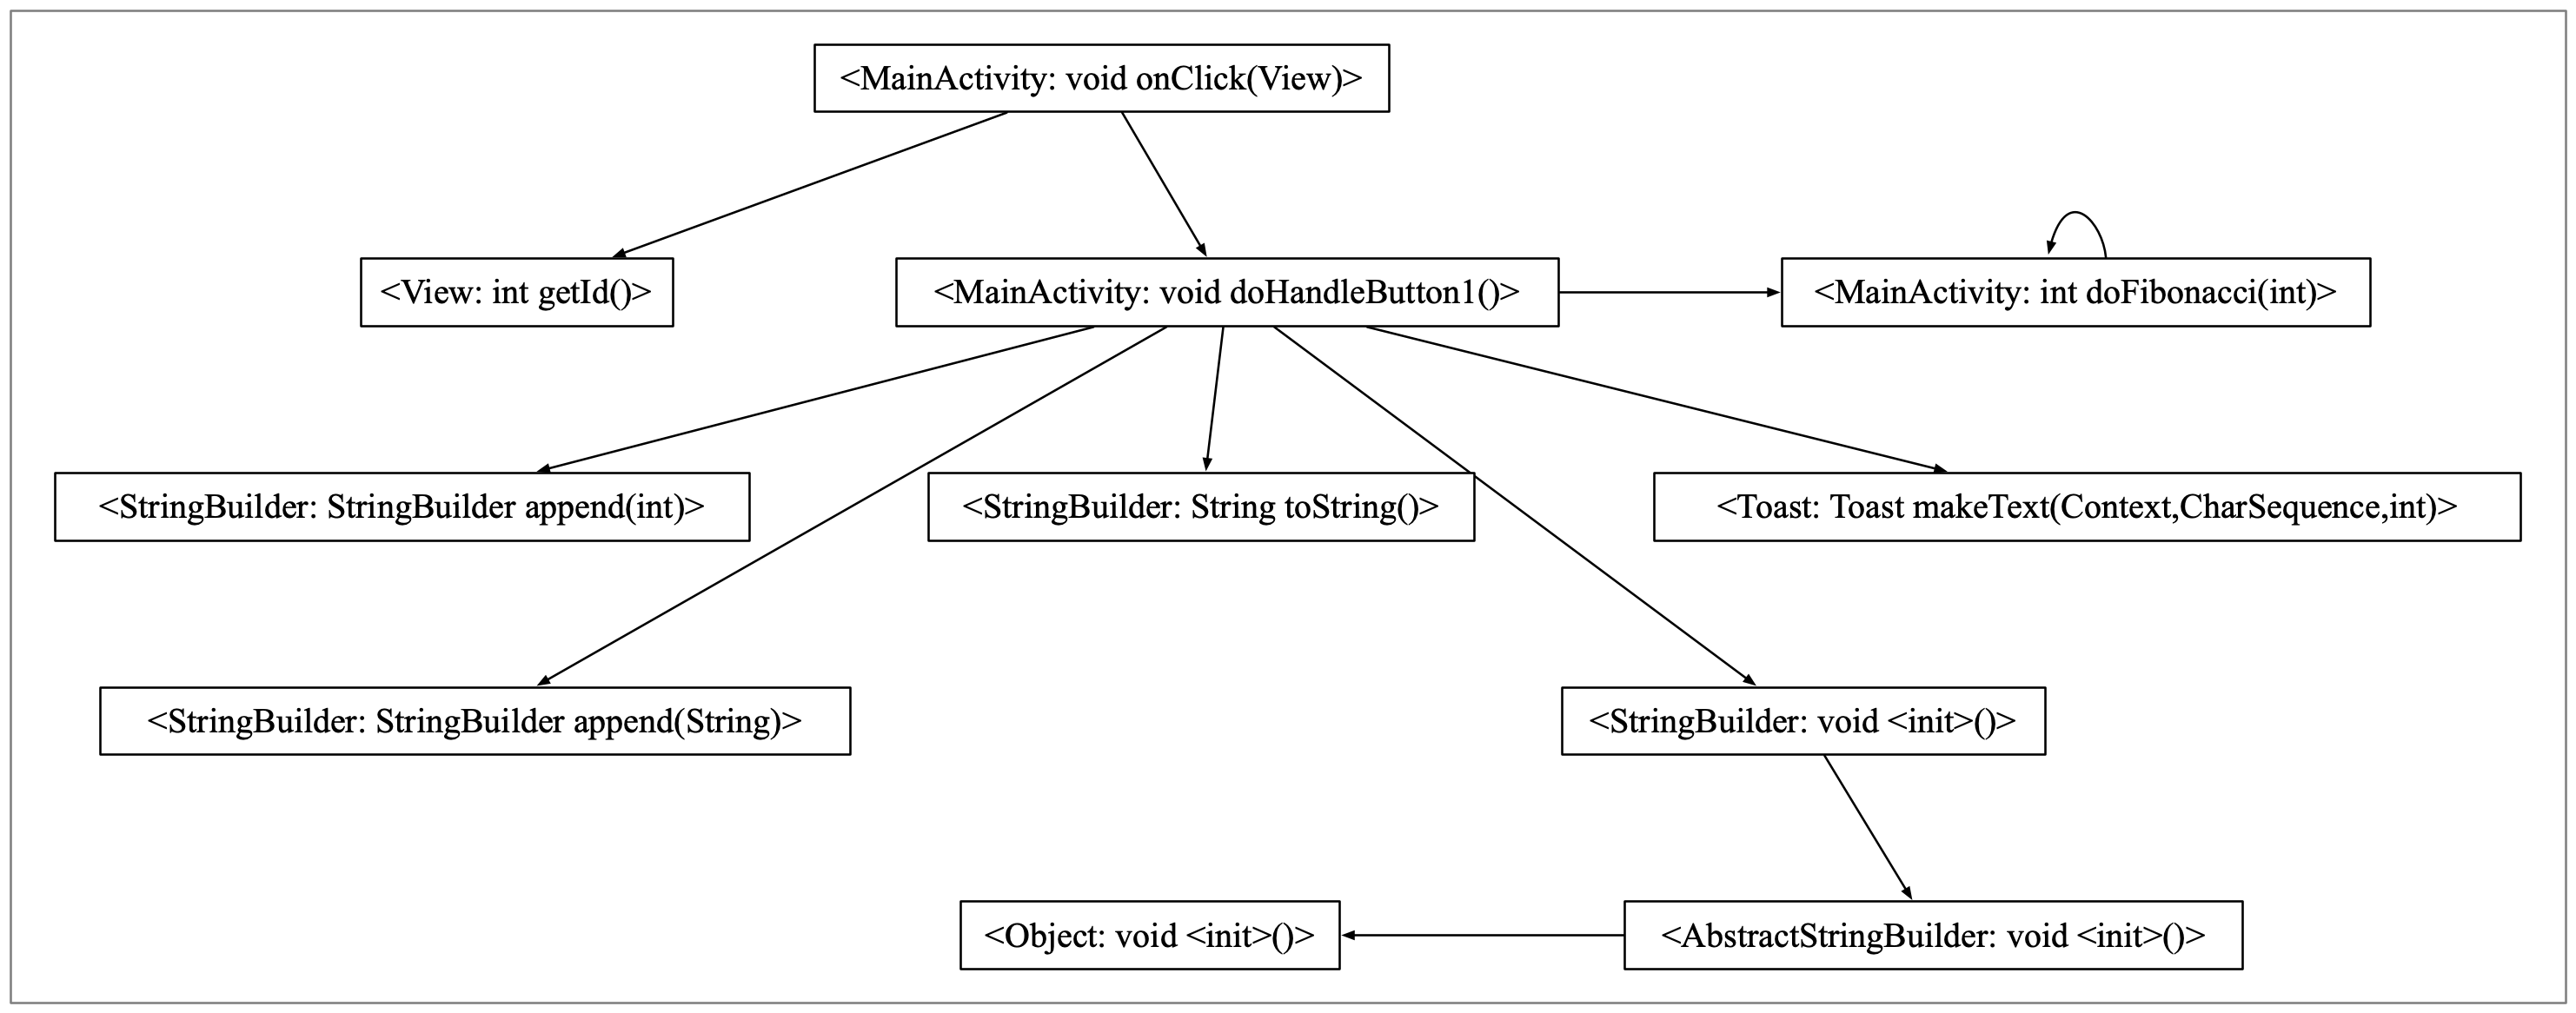
\includegraphics[width=\textwidth]{./Figures/FlowDroid-Fibonacci.png}
\caption{斐波拉契数列-FlowDroid生成的调用图}
\label{fig:flowdroid-result-Fibonacci}
\end{figure*}

\section{Activity的生命周期效果展示}


\section{多线程触发关系效果展示}

\begin{figure*}[ht]
	\centering
	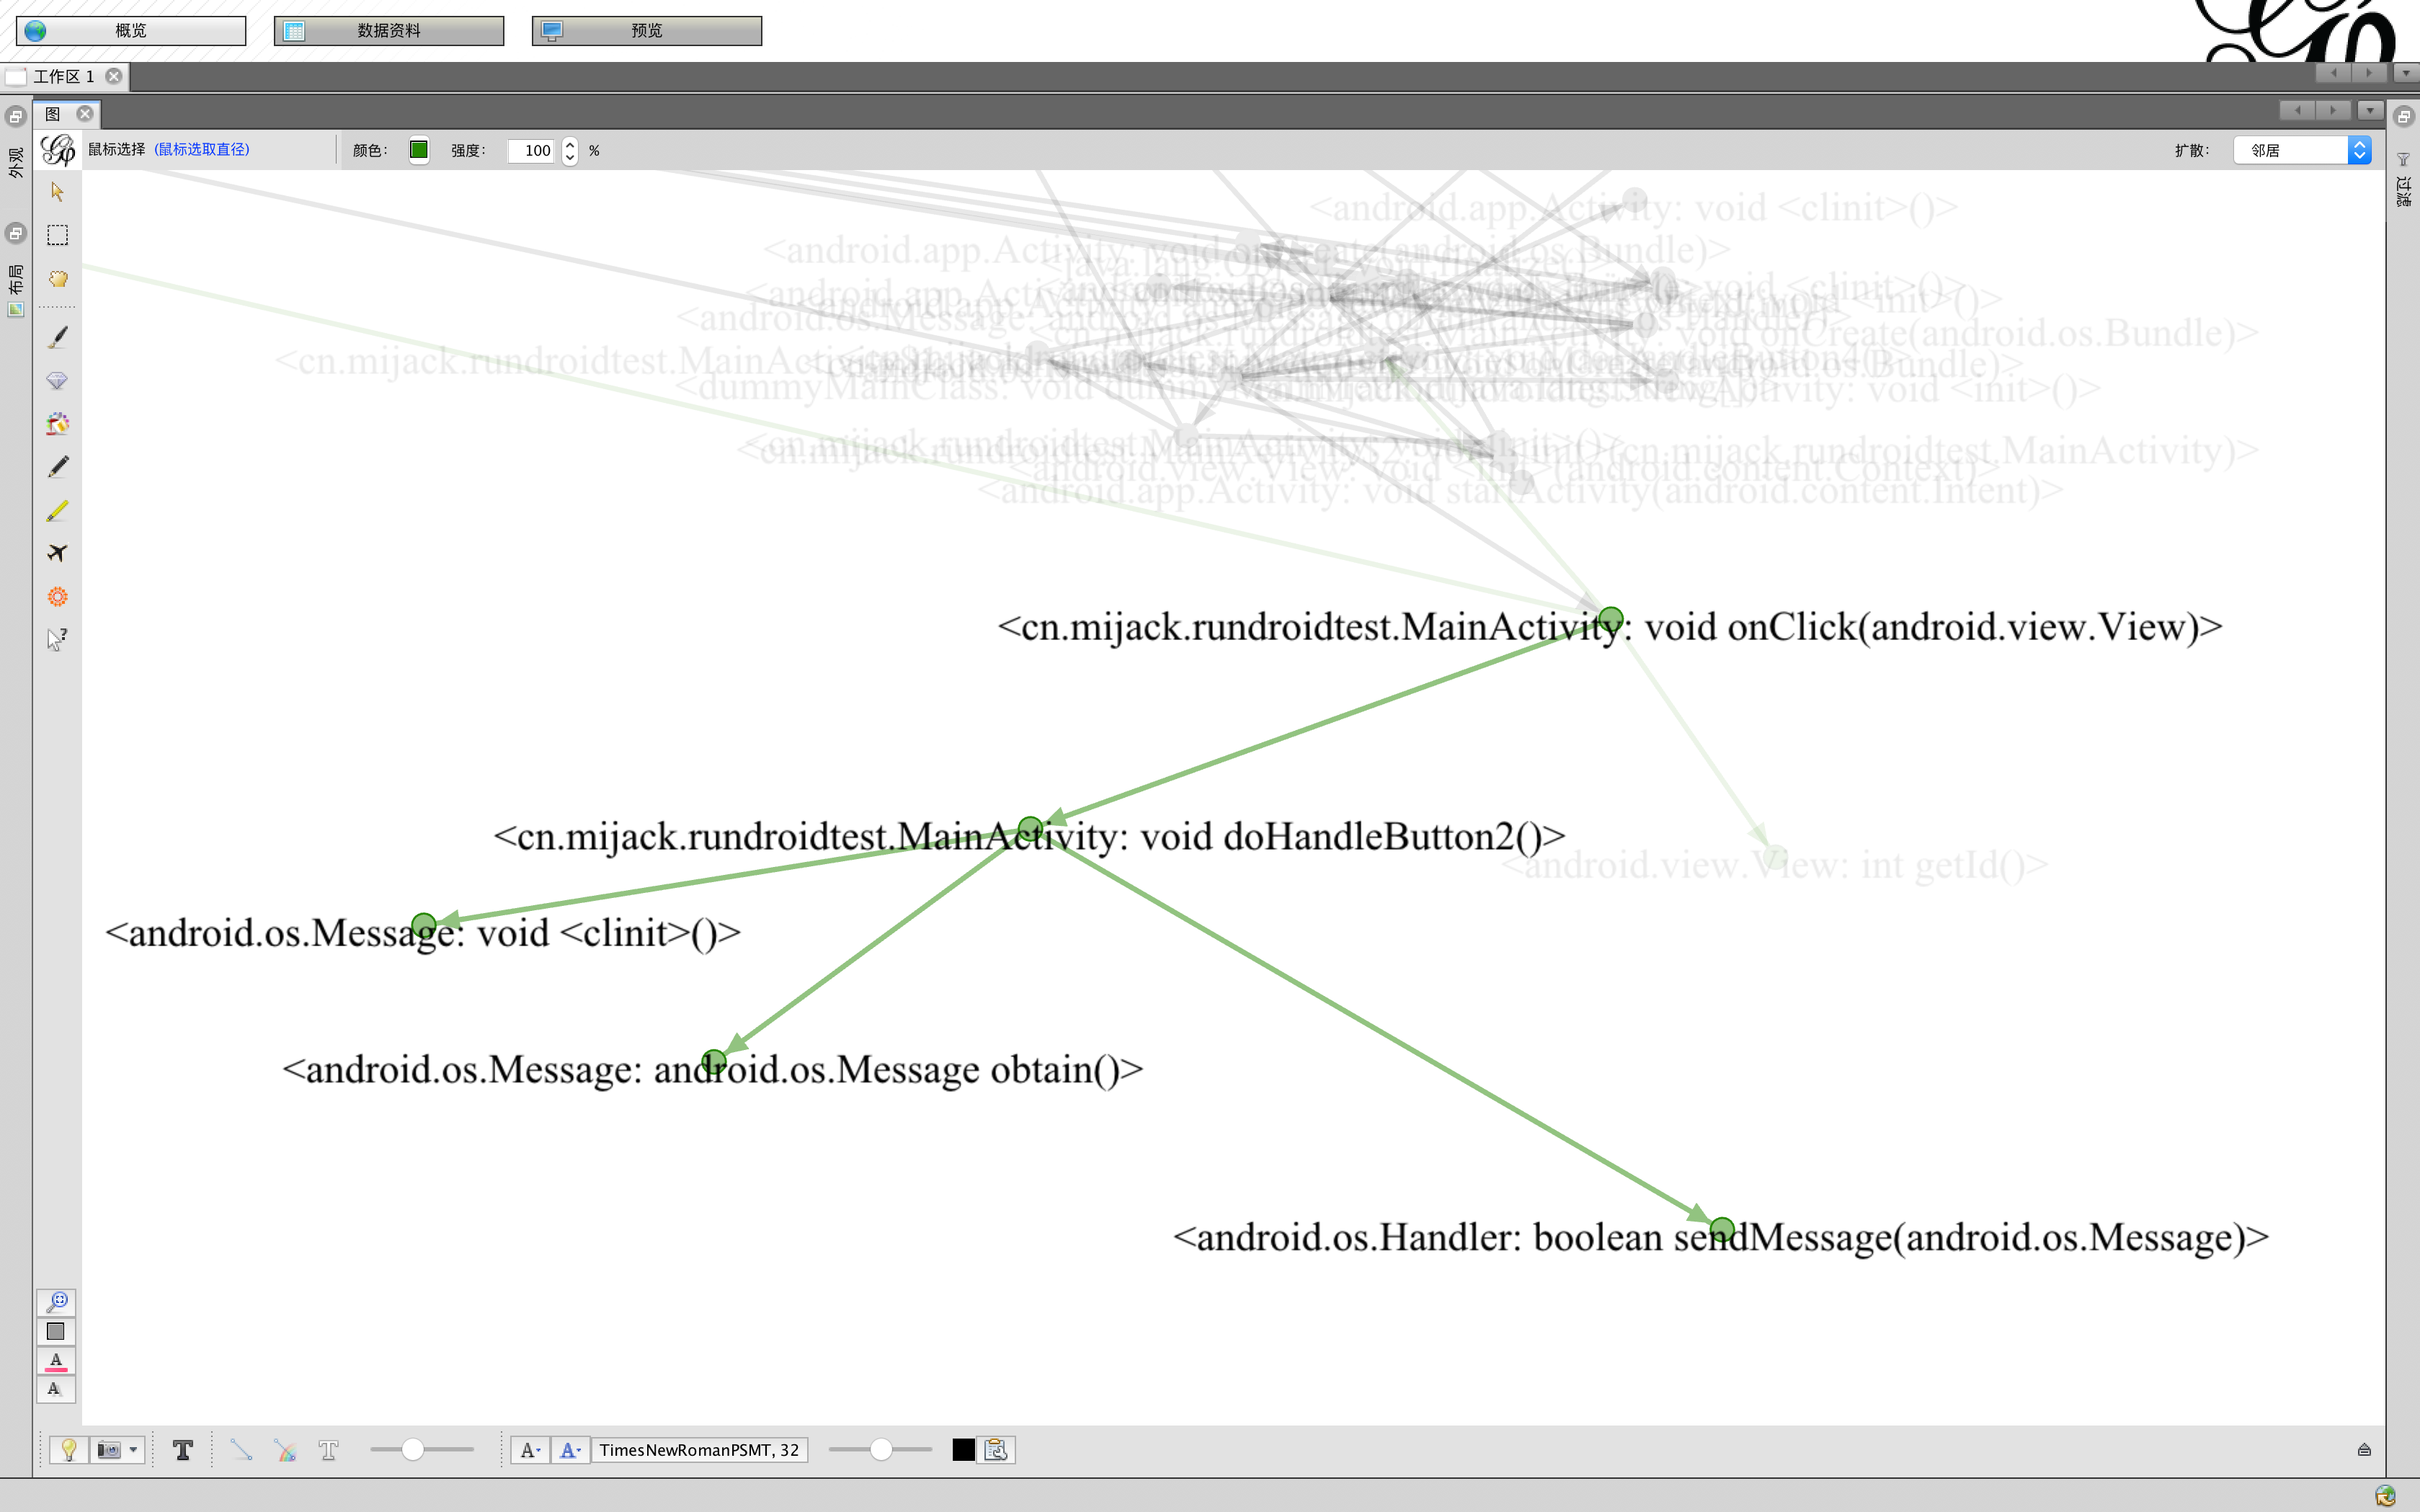
\includegraphics[width=\textwidth]{./Figures/FlowDroid-handler.png}
	\caption{Handler-FlowDroid生成的调用图}
	\label{fig:flowdroid-result-handler}
\end{figure*}
 \section{本章小结}
 
 将展示RunDroid系统生成的函数调用图的运行结果,并对函数调用图进行详细的阐述。
